% THIS IS SIGPROC-SP.TEX - VERSION 3.1
% WORKS WITH V3.2SP OF ACM_PROC_ARTICLE-SP.CLS
% APRIL 2009
%
% It is an example file showing how to use the 'acm_proc_article-sp.cls' V3.2SP
% LaTeX2e document class file for Conference Proceedings submissions.
% ----------------------------------------------------------------------------------------------------------------
% This .tex file (and associated .cls V3.2SP) *DOES NOT* produce:
%       1) The Permission Statement
%       2) The Conference (location) Info information
%       3) The Copyright Line with ACM data
%       4) Page numbering
% ---------------------------------------------------------------------------------------------------------------
% It is an example which *does* use the .bib file (from which the .bbl file
% is produced).
% REMEMBER HOWEVER: After having produced the .bbl file,
% and prior to final submission,
% you need to 'insert'  your .bbl file into your source .tex file so as to provide
% ONE 'self-contained' source file.
%
% Questions regarding SIGS should be sent to
% Adrienne Griscti ---> griscti@acm.org
%
% Questions/suggestions regarding the guidelines, .tex and .cls files, etc. to
% Gerald Murray ---> murray@hq.acm.org
%
% For tracking purposes - this is V3.1SP - APRIL 2009

\documentclass{acm_proc_article-sp}

\usepackage[utf8]{inputenc}
\usepackage [ ngerman ] { babel }

\newcommand{\mycirc}{$\circ~$}
\newcommand{\mycircOhne}{$\circ$}
\newcommand{\mycdot}{$\cdot~$}
\newcommand{\mycdotOhne}{$\cdot$}
\newcommand{\myin}{$\in~$}
\newcommand{\myMenge}[1]{$\mathbb{#1}$}
\newcommand{\myInfty}{$\infty~$}
\newcommand{\myInftyOhne}{$\infty$}
\newcommand{\myTiefstellen}[1]{$\mathrm{_#1}$}
\newcommand{\myZPStern}{\myMenge{Z}\myTiefstellen{p^*}}
\newcommand{\myRefGleichung}[1]{(\ref{#1})}

\newtheorem{defi}{Definition}
\newtheorem{beweis}{Beweis}

\begin{document}
	
	%TODO ...Problemlösenden Algorithmen für ...
\title{Algorithmische Zahlentheorie\titlenote{Genau Betrachtungen der Problemlösenden Algorithmen für Effiziente Primzahltests(Miller-Rabin-Test / AKS-Test) sowie den diskreten Logarithmus(Baby-Step-Giant-Step-Algorithmus / Index-Calculus-Algorithmus) sowie die dafür nötigen Grundlagen}}
\subtitle{Seminararbeit im Masterstudiengang Angewandte Informatik \\WS 2015/16 Hochschule Hannover
	\titlenote{ATM ka was man hier noch beschreiben könnte erstmal [TODO]}}

%
% You need the command \numberofauthors to handle the 'placement
% and alignment' of the authors beneath the title.
%
% For aesthetic reasons, we recommend 'three authors at a time'
% i.e. three 'name/affiliation blocks' be placed beneath the title.
%
% NOTE: You are NOT restricted in how many 'rows' of
% "name/affiliations" may appear. We just ask that you restrict
% the number of 'columns' to three.
%
% Because of the available 'opening page real-estate'
% we ask you to refrain from putting more than six authors
% (two rows with three columns) beneath the article title.
% More than six makes the first-page appear very cluttered indeed.
%
% Use the \alignauthor commands to handle the names
% and affiliations for an 'aesthetic maximum' of six authors.
% Add names, affiliations, addresses for
% the seventh etc. author(s) as the argument for the
% \additionalauthors command.
% These 'additional authors' will be output/set for you
% without further effort on your part as the last section in
% the body of your article BEFORE References or any Appendices.

\numberofauthors{2} %  in this sample file, there are a *total*
% of EIGHT authors. SIX appear on the 'first-page' (for formatting
% reasons) and the remaining two appear in the \additionalauthors section.
%
\author{
	% You can go ahead and credit any number of authors here,
	% e.g. one 'row of three' or two rows (consisting of one row of three
	% and a second row of one, two or three).
	%
	% The command \alignauthor (no curly braces needed) should
	% precede each author name, affiliation/snail-mail address and
	% e-mail address. Additionally, tag each line of
	% affiliation/address with \affaddr, and tag the
	% e-mail address with \email.
	%
	% 1st. author
	\alignauthor
	Marius Rohde\titlenote{Marius Rohde ... [TODO]}\\
	\affaddr{Hochschule Hannover}\\
	\affaddr{Fakultät IV - Wirtschaft und Informatik}\\
	\affaddr{30459 Hannover}\\
	\email{Marius.Rohde@stud.HS-Hannover.de}
	% 2nd. author
	\alignauthor
	Marcel Reichenbach\titlenote{Marcel Reichenbach wünscht allen Lesern und Leserinnen ein Frohes Weihnachten und einen guten Rutsch ins neue Jahr und sowie im nächsten Jahr bald Master zu sein}\\
	\affaddr{Hochschule Hannover}\\
	\affaddr{Fakultät IV - Wirtschaft und Informatik}\\
	\affaddr{30459 Hannover}\\
	\email{Marcel.Reichenbach@stud.HS-Hannover.de}
}


\maketitle
	
	\begin{abstract}
	%TODO Zusammenfassung
	Zusammenfassung ... [TODO]
\end{abstract}
	
	\section{Einleitung}
	Die algorithmische Zahlentheorie bildet die Grundlage der heutigen asymmetrischen Kryptographie und somit auch für einen Großteil des sicheren Datenverkehrs in Netzwerken. Ob Onlinebanking, digitale Signaturen oder virtuelle private Netzwerke, überall finden asymmetrische Verschlüsselungsalgorithmen Anwendung. Obwohl bereits Euklid ca. 300 v. Chr. zahlentheoretische Algorithmen entwickelt hat, konnte erst mit der asymmetrischen Verschlüsselung eine praktische Anwendung der Zahlentheorie gefunden werden. Zu den bedeutendsten Mathematikern, die sich mit der Zahlentheorie beschäftigten, gehören Euklid, Eratosthenes von Kyrene, Sun-Tse, Pierre de Fermat, Leonhard Euler, Carl Friedrich Gauß und David Hilbert. Trotz der langen Historie sind einige Fragen der Zahlentheorie wie z.B. die Unendlichkeit der Primzahlzwillinge oder die Goldbachsche Vermutung seit Jahrhunderten ungelöst. Erst 2002 konnten die drei indischen Wissenschaftler Manindra Agrawal, Neeraj Kayal und Nitin Saxena einen Beweis für die Existenz eines deterministischen Primzahltests liefern.\cite{Primes:is:in:P}
	
	Im folgenden werden die Grundlagen der Zahlentheorie eingeführt, um anschließend ausgewählte Algorithmen, die in der asymmetrischen Kryptographie eingesetzt werden, betrachten zu können. Zum Nachschlagen weiterer Informationen über Persönlichkeiten der Zahlentheorie mit historischer Einordnung bietet das Buch \cite{Elementare:Zahlentheorie} von Jochen Ziegenbalg einen guten Überblick.
	
	\section{Grundlagen}
	%TODO Grundlagen
	Grundlagen ... [TODO]
	
	\subsection{Algebraische Strukturen}
		In diesem Kapitel werden die algebraischen Strukturen: Halbgruppen, Gruppen, Ringe und Körper vorgestellt. Diese werden für ein späteres Kapitel benötigt. Die algebraischen Strukturen beschreiben ein abstraktes Rechnen mit Zahlen. Dies ermöglicht gezielter nur die Rechenregeln an sich zu untersuchen, unabhängig von der Rechengröße und der jeweiligen Operation. Ein Anwendungsbereich ist u. a. in der Kryptographie zu finden. 
	
		\subsection{Halbgruppen}
			%TODO siehe Text
			Eine Halbgruppe ist eine Menge M mit einer assoziativen Operation °. Assoziativgesetz: (a ° b) ° c = a ° (b ° c) für alle a, b, c € M. Das Zeichen ° ist Platzhalter für eine beliebige Operation. Der Wertebereich von ° ist eine Teilmenge von M so dass, a ° b € M für alle a, b €. Für das Zeichen ° werden auch die folgenden Operationszeichen verwendet: *, [MAL], +. Auch muss die Menge nicht zwangsläufig M sein. \textbf{[TODO Definition (Halbgruppe, Assoziativgesetz) S. 44]} Zum besseren verständnis konkrete Beispiele von Halbgruppen:
			
			\begin{itemize}
				\item N, Z, Q, R, C \textbf{[TODO noch die richtigen Symbole rein]} sind Halbgruppen mit der Addition als Operation, ebenso mit der Multiplikation.
				\item Wenn a ° b = |b - a| für alle a, b € Z, dann ist (Z, °) keine Halbgruppe. Da in diesem Fall (1 ° 2) ° 3 = 1 ° (2 ° 3) = 2 ist, aber 1 ° (2 ° 3) = 1 ° 1 = 0 ist.
			\end{itemize}
		
		\subsection{Monoide}
		
		
		\subsection{Gruppe}
		
		
		\subsection{Ringe}
		
		
		\subsection{Körper}
	
	\section{Primzahlen}\label{Kapitel Primzahlen}
	Natürliche Primzahlen werden definiert durch Zahlen > 1, die nur durch Eins oder sich selbst teilbar sind. Wie im Kapitel Primfaktorzerlegung gezeigt, können alle natürlichen Zahlen mit einer Multiplikation von Primzahlen erzeugt werden. Sie bilden sozusagen die Bausteine aller natürlichen Zahlen. Die Unberechenbarkeit, mit der sie auftreten, gibt Mathematikern schon seit Jahrtausenden Rätsel auf und ist ein Grundstein unserer heutigen Verschlüsselungsverfahren.
	In anderen Zahlensystemen als den natürlichen Zahlen ist die gewohnte Definition von Primzahlen nicht vollständig/korrekt. Sie sagt nur etwas über die Irreduzibelität eines Elements in einem Integritätsbereich aus. Da in den natürlichen Zahlen aber jedes irreduzibles Element auch prim ist, reicht diese Definition für \myMenge{N} aus.
	Für alle Integritätsbereiche gilt für die Primheit folgende Definition nach \cite{Algorithmische:Zahlentheorie}:
	
	Ein Element \myMathRM{p \in R\setminus(R^* \cup~\{0\})} heißt prim oder Primelement, wenn für alle \myMathRM{a, b \in R\setminus\{0\}} gilt:	
	\begin{displaymath}
		p~|~ab \Longrightarrow p~|~a~oder~p~|~b.
	\end{displaymath}
		
	Mit Hilfe der Primzahlen kann der Restklassenring \myMenge{Z}/m\myMenge{Z} spezialisiert werden. Ist m eine Primzahl p, so ist \myMenge{Z}/p\myMenge{Z} ein Körper und wird auch \myMenge{F}\myTiefstellen{p} bzw. \myMenge{GF}\myTiefstellen{p} bezeichnet.
	
	Neben den normalen Primzahlen gibt es weitere sogenannte Pseudoprimzahlen. Diese Zahlen verhalten sich bezogen auf einen Algorithmus genauso wie echte Primzahlen, sie sind jedoch zusammengesetzt. Ein Beispiel für solche Zahlen sind Carmichaelzahlen, die in einem späteren Kapitel thematisiert sind.

	Leider gibt es keine bekannten effizienten Verfahren, um Primzahlen zu generieren. Dennoch kann man Primzahlen recht einfach raten. Grundsätzlich ist es möglich, eine große Anzahl von Zahlen auszuschließen. Man denke an: nur ungerade Zahlen, die Teilungsgesetze und die Tatsache, dass alle Primzahlen > 3 in der Form 4k +1 oder 4k +3, k \myin \myMenge{N} vorliegen. Alle geratenen Zahlen müssen jedoch einem Primzahltest (vgl. Kapitel \ref{Effiziente Primzahltests}) zur Verifizierung unterzogen werden. In \cite{Algebraische:und:zahlentheoretische:Grundlagen:fuer:die:Informatik} ist beschrieben, wie ein Generierungsprozess erfolgen kann.

	\subsection{Primfaktorzerlegung}
	Jede natürliche Zahl größer als Eins, kann als Produkt von Primzahlen geschrieben werden. Dieser zentrale Satz wird als Fundamentalsatz der Zahlentheorie bezeichnet und kann auf jeden euklidischen Ring R angewendet werden. Eine Primfaktorzerlegung wird mit x \myin R, u \myin R*, \myMathRM{e_1, e_2, ..., e_m} \myin \myMenge{N} wie folgt definiert:	
	\begin{displaymath}
		x = u \cdot p^{e_1}_1 \cdot p^{e_2}_2 \cdot . . . \cdot p^{e_m}_m,
	\end{displaymath}
	wobei  \myMathRM{p_1 < p_2 < ... < p_m} Primelemente sind.
	
	Neben der Existenz einer solchen Primfaktorzerlegung ist auch die Eindeutigkeit, die durch das Vergleichszeichen \grqq kleiner als\grqq ~implizit angegeben ist, von entscheidender Bedeutung. In \cite{Einfuehrung:in:Algebra:und:Zahlentheorie} und \cite{Algorithmische:Zahlentheorie} wird die Existenz und Eindeutigkeit bewiesen.

	Die meisten kryptographischen Algorithmen bauen auf die ineffiziente Berechnung der Primfaktoren. Es ist zwar einfach, zwei Primzahlen miteinander zu multiplizieren, aber es ist schwer, aus der multiplizierten Zahl die beiden Primfaktoren zurückzugewinnen. Kennt man jedoch eine der beiden Primzahlen, so berechnet sich die zweite durch einfache Division. Zur Verschlüsselung ergibt sich damit die Idee einer sogenannten Falltür-Funktion, die die Primfaktoren mit Hilfe eines geheimen Hinweises schnell berechnen kann.
		
	\subsection{Satz von Euler und Kleiner Satz von Fermat}
	Die Vermutung vom kleinen Satz von Fermat wurde von Fermat im 17. Jahrhundert aufgestellt und von Euler bewiesen. Euler konnte zudem zeigen, dass der kleine Satz von Fermat nur ein Spezialfall für Primzahlen darstellt. Der Satz von Euler lautet:
	
	Sei m \myGroesserGleich 2 \myin \myMenge{N}. Dann gilt für jede zu m teilerfremde Zahl a \myin \myMenge{N}
	\begin{displaymath}
		a^{\varphi(m)} \equiv~1~mod~m.
	\end{displaymath}
	Denn wie in \cite{Algorithmische:Zahlentheorie} anhand der Gruppentheorie bewiesen, ist
	\begin{displaymath}
		a^{Ord(G)} = a^{|G|} = e,
	\end{displaymath}
	wobei G eine endliche Gruppe ist, a \myin G und e das Einselement (neutrales Element einer multiplikativen Gruppe). Da das Einselement in \myMenge{N} 1 ist, folgt: Kongruenz 1 modulo m. 
	
	Des weiteren ergibt sich mit 
	\begin{displaymath}
		\varphi(p) = Card((\mathbb{Z}/p\mathbb{Z})^*) = |\mathbb{F}^*_p| = p-1, p~prim
	\end{displaymath}
	sofort der kleine Satz von Fermat:
	\begin{displaymath}
		a^{p-1} \equiv~1~mod~p
	\end{displaymath}
		
	Mit dem Satz von Euler und Fermat kann nun ein erster primitiver Primzahltest definiert werden.  
	Für ein beliebiges 	a \myin \myMenge{N} mit 1 < a < m gilt:
	\begin{displaymath}
		a^{m-1} \not\equiv 1~mod~m \Longrightarrow nicht~prim
	\end{displaymath}
	Leider ist der fermatsche Primzahltest nur ein negativ Test, der eindeutig zeigen kann, dass eine Zahl nicht prim ist. Wenn der Test einer Zahl kongruent 1 modulo m ergibt, muss m also nicht prim sein. Eine Zahl, die für den Test prim ist, ist entweder eine echte Primzahl oder eine Pseudoprimzahl m zur Basis a.\cite{Elementare:Zahlentheorie}
		
	\subsection{Carmichaelzahlen}
	Da Pseudoprimzahlen die Primalität immer zu einer Basis aufweisen, liegt der Versuch nahe, andere Basen zu suchen, für die der fermatsche Test nachweisen kann, dass die vermeintliche Primzahl gar keine ist. Dies ist der Grundbaustein für probabilistische Primzahltests. Dennoch gibt es Zahlen, für die der fermatsche Test bei allen teilerfremden Basen kongruent eins Äquivalenz feststellt. Diese starken fermatschen Pseudoprimzahlen heißen Carmichaelzahlen.
	
	Carmichaelzahlen werden nach \cite{Algebraische:und:zahlentheoretische:Grundlagen:fuer:die:Informatik} so definiert:
	
	Eine zusammengesetzte Zahl m \myin \myMenge{N}, m \myMathRM{\geq} 3, heißt Carmichaelzahl genau dann, wenn für alle Basen a mit ggT(m, a) = 1 gilt: 
	\begin{displaymath}
		a^{m-1} \equiv 1~mod~m
	\end{displaymath}
	Die weiteren zwei folgenden Eigenschaften seien zudem genannt, da sie für den probabilistischen Primzahltest von Miller und Rabin von entscheidender Bedeutung sind.
	
	Eine zusammengesetzte Zahl m \myMathRM{\geq} 3 \myin N ist eine Carmichaelzahl, wenn m keine mehrfachen gleichen Primfaktoren enthält und für jeden Primfaktor p | m auch 
	\begin{displaymath}
		p-1~|~m-1
	\end{displaymath}
	gilt.	
	
	\subsection{Sieb des Eratosthenes}
	Das Sieb des Eratosthenes ist eines der ältesten bekannten Verfahren, um Primzahlen zu erhalten. Es berechnet für ein gegebenes n \myin \myMenge{N} alle Primzahlen p \myin \myMenge{N}, für die gilt 1 < p < n. Der Algorithmus iteriert dazu über alle nicht gestrichenen Zahlen von 1 bis \myMathRM{\sqrt{n}}. Als erstes wird die Zahl Zwei genommen, sie ist nicht gestrichen und somit eine Primzahl. Dann werden alle Vielfache von Zwei gestrichen (die geraden Zahlen). Anschließend sucht der Algorithmus die nächste nicht gestrichene Zahl. In diesem Fall ist es die Drei und es werden wieder alle Vielfache von drei gestrichen. Das Verfahren wiederholt sich, bis die Suche \myMathRM{\sqrt{n}} erreicht hat. Alle nicht gestrichen Zahlen sind die Primzahlen bis n. Die Abbildung \ref{ABBILDUNG_Primzahlen_100} illustriert die Primzahlen bis 100.
	Wie in \cite{Algebraische:und:zahlentheoretische:Grundlagen:fuer:die:Informatik} gezeigt, hat das Sieb des Eratosthenes eine subexponentielle Laufzeit, da die Laufzeit von der Länge der Eingabe abhängt. Aus diesem Grund eignet es sich nicht für einen praktischen Primzahltest.
	\begin{figure}
		\centering
		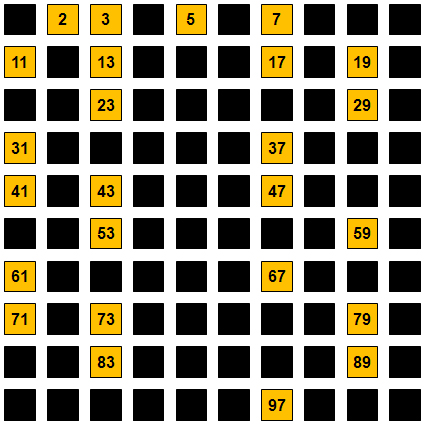
\epsfig{file=includes/images/primzahlen100.jpg, height=3in, width=3in}
		\caption{Primzahlen bis 100 Quelle: \cite{Mathe:Lexikon:SiebDesEratosthenes}}
		\label{ABBILDUNG_Primzahlen_100}
	\end{figure}
	
	\subsection{Effiziente Primzahltests} \label{Effiziente Primzahltests}
		Die in diesem Kapitel vorgestellten Algorithmen zum Erkennen von Primzahlen sind effiziente Algorithmen im Sinne der Komplexitätsklasse P und im Gegensatz zum fermatschen Test nicht anfällig für starke Pseudoprimzahlen. Dennoch unterscheiden sich die beiden vorgestellten Verfahren deutlich voneinander. Neben der Funktionsweise wird auch die Laufzeit gegenübergestellt.
		
		\subsubsection{Miller-Rabin-Test}
		 Der Miller-Rabin-Test ist ein probabilistischer Primzahltest und gehört zu den Montecarlo- Algorithmen. Im Gegensatz zum fermatschen Primzahltest ist der Miller-Rabin-Test nicht so anfällig für Carmichaelzahlen, denn es können immer Basen gefunden werden, die die Carmichaelzahlen entlarven. Dieser Test wird am häufigsten in Primzahlgeneratoren eingesetzt und hat damit die größte praktische Relevanz. Nach der Vorstellung des Tests werden die Unterschiede zum fermatschen Test herausgearbeitet.
		 
		 Der Test lautet wie folgt:
		 
		 Wenn m \myin \myMenge{N} > 9  eine ungerade Zahl und \myMathRM{m - 1 = 2^tn} mit ungeradem n ist, dann gilt für jede teilerfremde Zahl a \myin \myMenge{Z}:		 
	 	\begin{equation} \label{eq:Miller}
			a^n \equiv 1~mod~m~oder~\exists s \in \{0,..., t - 1\} : a^{2^sn} \equiv -1~mod~m
		\end{equation}
		dann ist m prim oder nicht prim.
		
		Aber wenn m nicht prim ist, so gilt außerdem für die Menge A aller zu m teilerfremden a, 0 < a < m die (\ref{eq:Miller}) erfüllen:
	 	\begin{displaymath}
		 	Card(A) \leq 1/4 \varphi(m)
	 	\end{displaymath}
	 	Durch diese zusätzliche Aussage kann eine Wahrscheinlichkeit angegeben werden, mit der die getestete Zahl prim ist. Wiederholt man den Test t mal, ergibt sich somit eine Wahrscheinlichkeit von \myMathRM{1/4^t}. Nach nur zehn Iterationen ist die Wahrscheinlichkeit für eine zusammengesetzte Zahl kleiner als \myMathRM{10^{-6}}.
	 	
	 	Um die Ausdrücke in (\ref{eq:Miller}) zu verstehen müssen folgende Vorüberlegungen gemacht werden.
	 	Jeder Körper \myMathRM{F^*_p} kann nach \cite{Algorithmische:Zahlentheorie} in die zwei Teile (Untergruppen) der Quadrate und nicht Quadrate geteilt werden. Jede dieser Gruppen besteht aus \myMathRM{Card(F^*_p)/2 = (p-1)/2} Elementen. Dies folgt aus der Tatsache, dass \myMathRM{x^2 \equiv~a~mod~p} in \myMathRM{F^*_p} nur die Lösungen +1 oder -1 hat. Ein Element ist ein Quadrat, wenn es gleich dem quadratischen Rest eines \myMathRM{x^2~mod~p} ist.
	 	
	 	Eine weitere Überlegung ergibt sich aus dem umgekehrten Satz des Eulerkriteriums, der wie folgt lautet:
	 	Sei \myMathRM{m \geq 3} eine ungerade ganze Zahl, so dass (m - 1)/2 ungerade ist.
	 	Es gilt dann für jede zu m teilerfremde ganze Zahl a
	 	\begin{displaymath}
		 	a^{(m-1)/2} \equiv~^+_-1~mod~m,
	 	\end{displaymath}
	 	so dass m eine Primzahl ist.
	 	
	 	Wenn (m - 1)/2 gerade ist, kann diese Aussage nicht getroffen werden. Für den Fall, dass m eine Carmichaelzahl ist, ist auch \myMathRM{m - 1 = 2^{s_i}u_i(p_i - 1)} , da alle Primfaktoren m-1 teilen, wobei \myMathRM{u_i} ungerade ist. Es gilt dann O.B.d.A mit \myMathRM{s_1 \leq s_2 \leq . . . \leq s_r~und~s = s_1}:
 		\begin{displaymath}
	 		a^{(m-1)/2^s} \equiv1 ~fuer~alle~a \in \mathbb{Z}^*_m
 		\end{displaymath}
 		Anschließend müssen wie in \cite{Algorithmische:Zahlentheorie} durchgeführt, mehrere Fallunterscheidungen für gerade und ungerade vielfache von \myMathRM{(a^{(m-1)/2^{s+1}})} durchgeführt werden. Dabei können die Ergebnisse der Kongruenzen in Teilmengen eingeteilt werden. Die Kardinalität der Mengen gibt dabei die Wahrscheinlichkeit der Zusammengesetzten Zahlen vor.
 		
 		Etwas abstrakter dargestellt zielt der Test darauf ab, im Gegensatz zu dem fermatschen Test, die Quadratwurzeln der Carmichaelzahlen in dem Primzahlkriterium zu berücksichtigen. Durch diese Erweiterung kommt es nur noch maximal bei einem Viertel der Basen zur Annahme, es handle sich um eine Primzahl.
 		
 		Wie in \cite{Algebraische:und:zahlentheoretische:Grundlagen:fuer:die:Informatik} angegeben, benötigt der Test, da die Exponentiation effizient berechenbar ist, O(t * (log m)) arithmetische Operationen und O(t * (log m)\myMathRM{^3}) Bit Operationen bezogen auf die Eingabelänge von m. Damit liegt der Test in der polynomialen Laufzeitklasse.
 		
 		Eine interessante Aussage die in \cite{Algorithmische:Zahlentheorie} getroffen wird, ist dass der Miller-Rabin-Test unter Annahme der Riemannschen Vermutung zu einem deterministischen polynomialen Test wird.
 		
 		%TODO Hier Pseudocode


		\subsubsection{AKS-Test}
		Der 2004 von M. Agrawal, N. Kayal und N. Saxena entwickelte AKS-Test \cite{Primes:is:in:P} ist ein deterministischer in polynomialer Zeit durchführbarer Primzahltest. Bei diesem Test stellt die Rechnung in einem Polynomring (\myMenge{Z}/m)[X] den größten Unterschied zu den bisherigen Tests da. Besonders wertvoll ist hier die notwendige und hinreichende Bedingung für die Primmalität des folgenden Satzes. 
		
		Der Satz lautet in \cite{Algorithmische:Zahlentheorie} wie folgt:
		Sei m > 1 eine natürliche Zahl und a eine zu m teilerfremde ganze
		Zahl. Genau dann ist m prim, wenn
		\begin{displaymath} 
			(X + a)^m \equiv X^m + a~mod~m
		\end{displaymath}
		
		Dieser Satz ist natürlich noch nicht schneller als die Probedivision bis \myMathRM{\sqrt{m}}, aber folgende Erweiterungen führen zu einem polynominelle Laufzeitverhalten. Die Idee hinter der Erweiterung ist, ein Polynom zu finden, das mit getestet wird und dadurch die Laufzeit reduziert. Ein solches Polynom ist \myMathRM{P(x) = x^r - 1}, r ist prim . Mit diesem Zusatz ist der Test wiederum nur ein notwendiges Kriterium für eine Primzahl. Dies kann verhindert werden, indem versucht wird, eine Menge Zahlen zu finden, in der mindestens ein Element für eine beliebige zusammengesetzte Zahl m das Kriterium nicht erfüllt. Diese Menge kann angegeben werden und lautet wie folgt:
		\begin{displaymath}
			A(r,m) = \{1, 2, . . . , 2 * \lfloor log~m *\sqrt{\varphi(r)} \rfloor\}
		\end{displaymath}
		Anders ausgedrückt muss jedes Element in der Menge A(r,m) die weiter unten angeführte Bedingung (\ref{eq:AKS}) erfüllen, damit m prim sein kann.
		
		Mit diesen Überlegungen kann im folgenden der Satz von Agrawal, Kayal und Saxena nach \cite{Algorithmische:Zahlentheorie} aufgestellt werden.
		
		Sei m > 1 eine ungerade Zahl. Weiter sei r eine Primzahl mit folgenden Eigenschaften:
		
		1. m hat keinen Primteiler \myMathRM{\leq} r.
		
		2. \myMathRM{ord_{(\mathbb{Z}/r)^*}(m) > (log_2 m)^2}.
		
		Gilt dann für alle \myMathRM{a = 1, 2, . . . , A:= \lfloor \sqrt{r}~log_2~m \rfloor}
		\begin{equation} \label{eq:AKS}		
			(X + a)^m \equiv X^m + a~mod~(m,X^r - 1),
		\end{equation}
		so ist m eine Primzahlpotenz, d.h. m = \myMathRM{p^k}, p prim, k \myMathRM{\geq} 1.
		
		Wie in \cite{Algorithmische:Zahlentheorie} und \cite{Algebraische:und:zahlentheoretische:Grundlagen:fuer:die:Informatik} beschrieben, lässt sich der vollständige Test so ausdrücken:
		
		Sei \myMathRM{m > 2^{24}} eine ganze Zahl. Um zu entscheiden, ob m prim ist, gehe man
		wie folgt vor:
		
		1. Im Intervall \myMathRM{(log_2~m)^2 < r < (log_2~m)^5} suche man nach einer Primzahl r mit
		r \myNichtTeiler m und \myMathRM{ord_{(\mathbb{Z}/r)^*}(m) > (log_2~m)^2}.
		Falls es kein solches r gibt, ist m nicht prim.
		
		2. Man vergewissere sich, dass m keinen Primteiler \myMathRM{p \leq r} besitzt.
		
		3. Für alle ganzen Zahlen a mit \myMathRM{1 \leq a \leq  \lfloor \sqrt{r}~log_2~m \rfloor} überprüfe man die Kongruenz (\ref{eq:AKS}).
		Ist diese Kongruenz auch nur für ein einziges a nicht erfüllt, ist m nicht prim.
		
		4. Hat m die Tests 1. bis 3. bestanden, ist m prim oder eine Primzahlpotenz.
		Man hat deshalb noch auszuschließen, dass sich m als Potenz \myMathRM{m = n^k} einer
		ganzen Zahl n mit einem Exponenten \myMathRM{k \geq 2} darstellen lässt.
		
		Wie in \cite{Algorithmische:Zahlentheorie} und \cite{Algebraische:und:zahlentheoretische:Grundlagen:fuer:die:Informatik} gut dargestellt, beträgt die Gesamtlaufzeit des Algorithmus unter bewiesenen Annahmen \myMathRM{O(log^{7,5} m)}. Schritt 3 spielt bei der praktischen Laufzeitbetrachtung die größte Rolle, da hier sehr große Polynome miteinander verrechnet werden müssen. Leider eignet sich der AKS-Test dadurch nicht für die Praxis. Für die theoretische Betrachtung war die Entdeckung des AKS-Test jedoch ein großer Erfolg, da nach sehr langer Zeit bewiesen werden konnte, dass die Primzahlerkennung in polynomieller Zeit durchführbar ist.
		
	
	\section{Diskreter Logarithmus}
	%TODO Diskreter Logarithmus
	Diskreter Logarithmus ... [TODO]
	
	\subsection{Elliptischen Kurven Grundlagen}
		
		Eine Elliptische Kurve ist eine ebene Kurve und durch nachfolgender Gleichung beschrieben: [TODO Gleichung von S. 153 aus \cite{Kryptographie:und:IT-Sicherheit}] 
		
		$y^2 = x^3 + ax +b$
		
		Addition von Punkten: Das Verknüpfen von zwei Punkten auf einer elliptischen Kurve ergibt wieder einen Punkt auf der Kurve und ist wie folgt geometrisch definiert:
		
		Definition: Durch die gegebenen Punkte P und Q wird eine Gerade gelegt, welche die Kurve in 
		einem dritten Punkt R schneidet. Dieser wird anschließend an der x-Achse 
		gespiegelt. Als Ergebnis erhält man den Punkt S, welcher als Addition von P und Q 
		bezeichnet wird. \cite{Information:und:Kommunikation}
		
		Mit Addition ist das Verknüpfen von zwei Punkten gemeint, man könnte es auch als Multiplikation bezeichnen.\cite{Information:und:Kommunikation}
		
		[TODO Bild von S. 252 \cite{Information:und:Kommunikation}]
		
		
		Die so definierte Addition ist kommutativ, zur Erinnerung: P + Q = Q + P.
		
		Damit die Additionsoperation, die wir definieren werden, für beliebige Punkte 
		der Kurve durchführbar ist, darf die Kurve sich nicht selbst schneiden (wie in dem Fall a= 3, 
		b=2 in Abb. 4-3). Bei so einer Kurve würde man die Addition nicht durchführen können, falls 
		der Schnittpunkt involviert wäre. Der Grund dafür wird bei der geometrischen Definition der 
		Addition  klar werden.\cite{Kryptographie:und:IT-Sicherheit}
		
		
		
		[TODO die zwei Spezialfälle]
		Nun können bei einer Addition von zwei Punkten die nachfolgenden Spezialfälle auftreten:
		
		\begin{itemize}
			\item Wenn für die beiden zu Addierenden Punkten Q = P gilt, wird die Tangente an der Kurve im Punkt P verwendet. Dabei entsteht der der Schnittpunkt mit der Kurve in R und durch Spiegelung resultiert daraus S = P + P = 2P
			\item Sollten die x-Koordinaten beider zu addierender Punkte gleich sein, so dass (XQ = XP) gilt, entsteht eine vertikale Gerade und die Kurve wird kein weiteres mal geschnitten. Für diesen Fall wird die elliptische Kurve um einen weiteren Punkt O\textbf{[TODO anderes Symbol]}, welcher im Unendlichen liegt, ergänzt. Die Addition von Punk P mit O\textbf{[TODO anderes Symbol]} ist so definiert das man wiederum P als Ergebnis erhält (P + O\textbf{[TODO anderes Symbol]} = P). Somit ist O\textbf{[TODO anderes Symbol]} das neutral Element der Addition. Es gilt also: P + Q = O\textbf{[TODO anderes Symbol]} wenn die x-Koordinaten von P und Q gleich sind. Daraus folgt das Q das inverse Element vo P ist und es gilt: Q = -P.
		\end{itemize}
		
		Addition mit einem Skalar: Die Addition von einem Punkt mit einem Skalar k \myin {1, 2, 3 ...} wird als wiederholte Addition definiert. Beispiel: kP = P + P + ... + P.
		
		Eine  Gerade  durch  zwei  Punkte  der 
		elliptischen Kurve muss diese also in einem dritten Punkt schneiden. \cite{Information:und:Kommunikation}		
		
		
		Die Menge aller Punkte (x, y) die die nachfolgende Gleichung erfüllen. Wichtig dabei ist das die Kurvenparameter a und b so gewählt sind das die partiellen Ableitungen nach x und nach y auf keinem Punkt der Kurve gleichzeitig null sind.\cite{Information:und:Kommunikation}
		
		
		
		
		In diesem Kapitel sollen nur die Grundlagen von Elliptischen Kurven näher gebracht werden um so die ECC-Kryptographie verstehen zu können. Um die Funktionsweise der Elliptischen Kurven zu verstehen ist dafür eine sehr komplexe Mathematik notwendig. Innerhalb dieser Seminararbeit kann diese Thema nicht tiefer durchleuchtet werden und es sei ihr auf die Folgende Literatur verwiesen. 
		
		
		
		Asymmetrische Verschlüsselungsverfahren basieren auf Einwegfunktionen. Wobei es nicht allzu schwierig ist k \mycdot P zu Berechnen allerdings ist das Berechnen von k aus k \mycdot P und P sehr aufwendig. Anzumerken ist das diese aussage allerdings bis heute noch nicht bewiesen wurde.
		
		
		Motivation: Der Vorteil des ECC-Verfahrens im vergleich zum RSA-Verfahren, ligt darin das die Schlüssellänge deutlich kürze ausfallen kann ohne dabei "Sicherheit" zu verlieren. Ein RSA-Schlüssel mit 1024 Bit ist etwa so sicher wie ein Schlüssel mit elliptischen Kurven mit ca. 160 Bit. Dazu kommt das der Rechenaufwand und der Speicherbedarf beim ECC-Verfahren wesentlich geringer ist als beim RSA-Verfahren. So kann ECC in Smartcards und Mobiltelefonen genutzt werden.\cite{Information:und:Kommunikation}
		
		
		Rechnen in einem Endlichen Körper: Bei der Addition und Multiplikation in endlichem Körpern sind diese so definiert, dass das Ergebnis immer wider ein Element des endlichem Körpers ist. Sollte bei der Addition oder Multiplikation von zwei Elementen den Zahlenbereich des endlichen Körpers verlassen muss eine weitere Operation durchgeführt werden: \textit{mod}. Der Resultierende Rest ist dann wieder innerhalb des endlichen Körpers. Für die Addition besitzt jedes Element ein inverses Element -a, damit gilt für die Subtraktion: b - a = b + (-a). Bei der Multiplikation ist das inverse Element $a^-1$, damit gilt für die Division: b / a = b \mycdot $a^1$. Siehe auch konkretes Beispiel in \cite{Information:und:Kommunikation} S. 154 - 257.
		
		Um elliptische Kurven für kryptologische Anwendungsfälle zu nutzen muss die Ordnung eines Punktes, welches auf der Kurve liegt berechnet werden. Definition: Die Ordnung eines Punktes ist die Anzahl der Punkte, die durch fortwährender Addition dieses Punktes, erzeugt werden. Beispiel P + P = 2P -> 2P +P = 3P -> ... -> xP + P = (x+1)P . P ist dabei immer ein Punkt auf der elliptischen Kurve. Irgendwann ist xiP = O\textbf{[TODO anderes Symbol]} und damit hat der Punkt P die Ordnung xi.
		
		Schlüsselaustausch  mit elliptischen  Kurven: Zuerst muss der Körper bestimmt werden und eine elliptische Kurve, dazu wählt man ein große Primzahl und die Kurvenparameter a und b. Weiter wird nun ein Erzeugerpunkt G vereinbart, dabei soll die Ordnung des Punktes G möglichst groß und eine Primzahl sein. A wählt eine geheime ganze Zahl nA welche kleiner sein muss als n und berechnet daraus den öffentlichen Schlüssel PA = nA \mycdot G. Teilnehmer B mach das gleich jeweils mit nB und PB. PA und PB können nun über eine unsichere Leitung ausgeschaut werden. Nun kann Teilnehmer A den Schlüssel K = nA \mycdot PB berechnen. B berechnet ebenfalls K nur mit nB und PA. So habe dabei ein und das selbe geheime K berechnet. Angreifer müsste
		
		Beweis: Es folgt der Beweis das A und B wirklich das gleiche K berechnet haben müssen: A berechnet K = nA \mycdot PB. Für PB wurde ursprünglich von Teilnehmer B berechnet mit nB \mycdot G. Die kann in die berechnung für K in PB eingesetzt werden so das daraus folgt: K = nA \mycdot PB = nA \mycdot (nB \mycdot G). Das gleiche Prinzip angewendet für die Berechnung von K von Teilnehmer B ergibt: K = nB \mycdot PA = nB \mycdot (nA \mycdot G). Unter Berücksichtigung des Assoziativgesetzes können diese beiden Gleichungen, gleich gesetzt werden: nA \mycdot (nB \mycdot G) = nB \mycdot (nA \mycdot G)
	
	\section{Fazit}
	Verschlüsselung von Daten ist aus der heutigen vernetzten Welt nicht mehr wegzudenken. Aus diesem Grund sind heutige Verschlüsselungstechniken, die auf Faktorisierung von Primzahlen oder dem diskreten Logarithmus-Problem beruhen, zum Standard geworden. Diese Ausarbeitung hat in Kapitel \ref{Kapitel Grundlagen} Grundlagen-Wissen u.a. über algebraische Strukturen, den Euklidischen Algorithmus, sowie zur Euler’schen \myPhi -Funktion vermittelt. Weiter wurde auch ein kleiner Teilbereich aus den elliptischen Kurven vorgestellt, um die nötigen Grundlagen für das ECC zu schaffen. In Kapitel \ref{Kapitel Primzahlen} wurden die Primzahlen genauer analysiert. Dabei ist die Primfaktorzerlegung essenziell für die Zahlentheorie und ermöglichen erst kryptographische Algorithmen, die auf eine ineffiziente Berechnung der Primfaktoren aufbauen.
	
	Das grundlegende Problem vom diskreten Logarithmus wurde in Kapitel \ref{Kapitel Diskreter Logarithmus} ausführlich erläutert. Des weiteren wurden Algorithmen vorgestellt, mit dessen Hilfe es möglich ist, den diskreten Logarithmus zu berechnen. Besonders der Index-Calculus-Algorithmus ist den allgemein verwendbaren Algorithmen deutlich überlegen, denn dieser hat eine Laufzeit von etwa $O(exp(\sqrt[]{2 \cdot ln~p \cdot ln~ln~p}))$. Eine genaue Beschreibung dieses Algorithmus ist dem Buch \cite{Einfuehrung:in:die:Kryptographie} zu entnehmen. Dieser ist auch dafür mitverantwortlich, weswegen elliptische Kurven gegenüber den multiplikativen Gruppen der endlichem Körper für kryptographische Anwendungsfälle \myAnfuehrungszeichen{sicherer} sind. Der Baby-Step-Giant-Step-Algorithmus kann sowohl für das DLP sowie für das ECDLP eingesetzt werden, besitzt allerdings nur eine Laufzeit von $O(\sqrt[]{p-1})$. Der Index-Calculus-Algorithmus hingegen lässt sich nicht auf elliptischen Kurven umschreiben. Hier bleiben nur die wesentlich langsameren allgemeinen Verfahren.\cite{Mathematisch:fuer:fortgeschrittene:Anfaenger}

	\begin{figure}
		\centering
		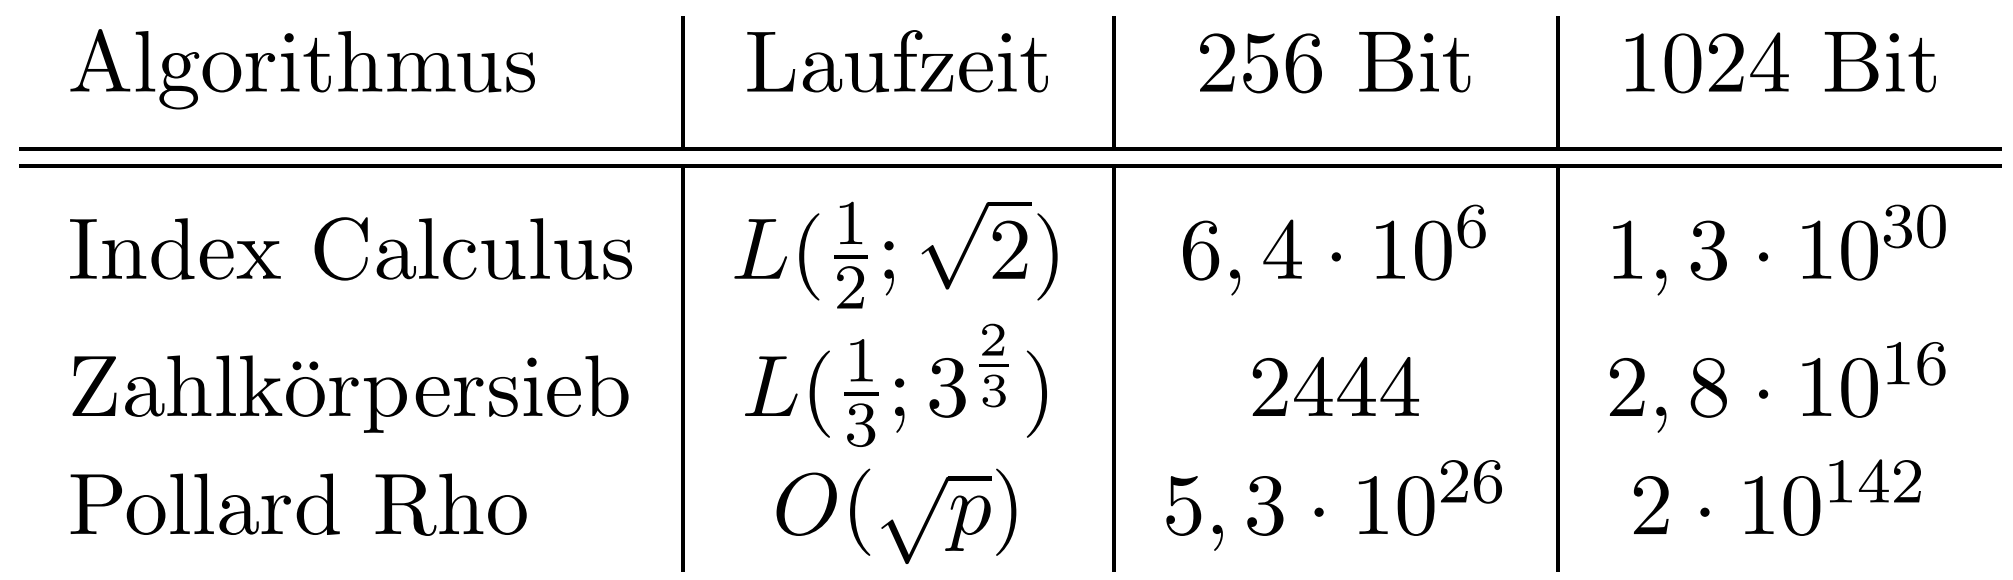
\includegraphics[width=0.4\textwidth]{includes/images/LaufzeitenDLP.PNG}
		\caption{Laufzeiten von Algorithmen für DLP (in Jahren bei eine Milliarde Berechnungen pro Sekunden)~\cite{DLP:ECDLP:Probleme:und:Loesungen}}
		\label{fig_LaufzeitenDLP}
	\end{figure}
	
	\begin{figure}
		\centering
		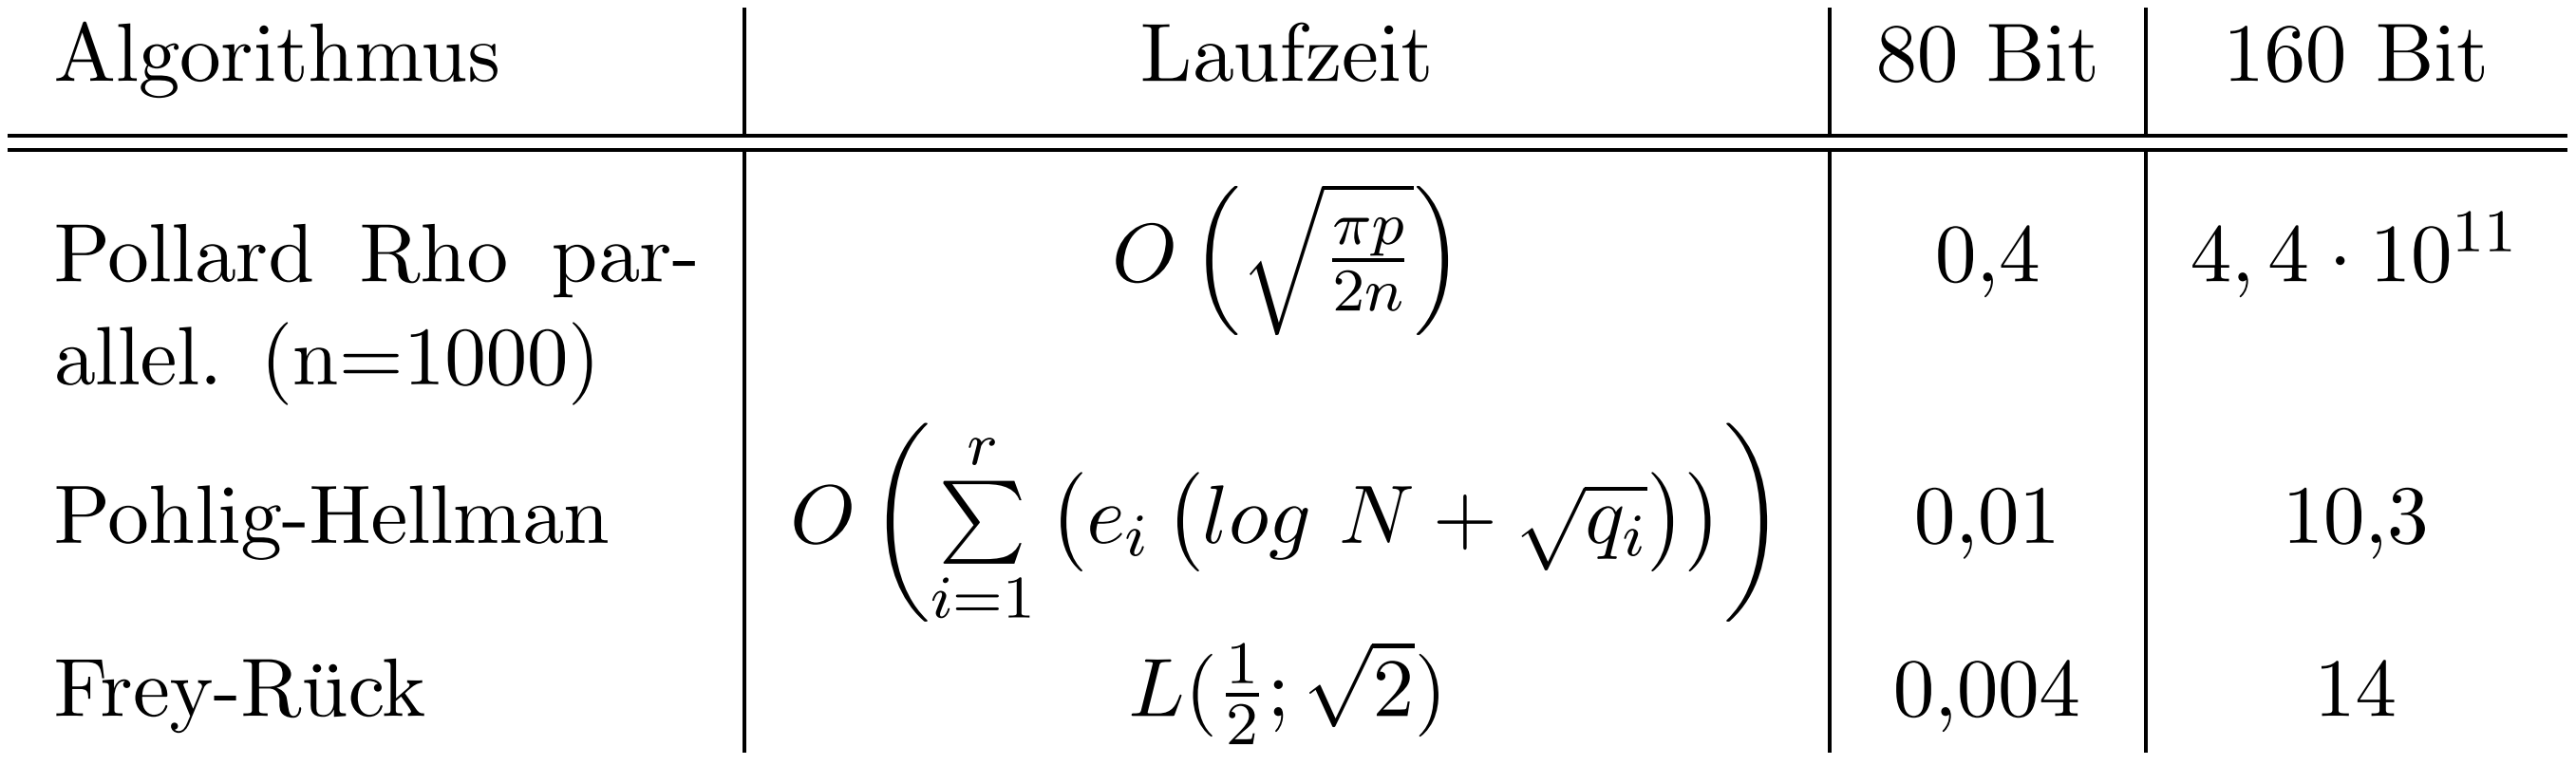
\includegraphics[width=0.5\textwidth]{includes/images/LaufzeitenECDLP.PNG}
		\caption{Laufzeiten von Algorithmen für ECDLP (in Jahren bei eine Milliarde Berechnungen pro Sekunden)~\cite{DLP:ECDLP:Probleme:und:Loesungen}}
		\label{fig_LaufzeitenECDLP}
	\end{figure}

	Bezüglich der Sicherheit von heutigen kryptographischen Verfahren muss man sich aktuell keine Sorgen machen, zumindest wenn die Mindestanforderungen bezüglich der Größe des Körpers und der Schlüssellänge eingehalten werden. Bei zu kleinen Schlüssellängen ist auch bei der besten Verschlüsselung heutzutage keine Sicherheit gegeben. Dies zeigen auch noch einmal die Abbildungen \ref{fig_LaufzeitenDLP} und \ref{fig_LaufzeitenECDLP}, mit den entsprechenden hochgerechneten Laufzeiten in Jahren, für Algorithmen zum Lösen des DLP und des ECDLP.
	
	Der Höhepunkt im Bereich der Verschlüsselung kann noch nicht erreicht sein. Noch schnellere und effizientere und somit \myAnfuehrungszeichen{sicherere} Verschlüsselungstechniken werden benötigt, um auch zukünftigen Anforderungen gerecht zu werden. Denn laut Peter W. Shor existieren bereits die nötigen Algorithmen, um sämtliche heutigen Verschlüsselungen zu brechen. Diese stellt er in \cite{Algorithms:for:Quantum:Computation:Discrete:Logarithms:and:Factoring} vor. Diskrete Logarithmen können in polynomialer Zeit berechnet werden, es muss nur noch gelingen einen genügend großen Quantencomputer zu bauen.
	
	\bibliographystyle{abbrv}
\bibliography{AlgorithmischeZahlentheorie}
	
	\section{Anhang}
	%TODO Anhang
	Anhang ... [TODO]

\end{document}
